\section{Antenna Design 1 - Monopole}

\begin{figure}[htbp]
    \begin{subfigure}[b]{0.49\linewidth}
        \centering
        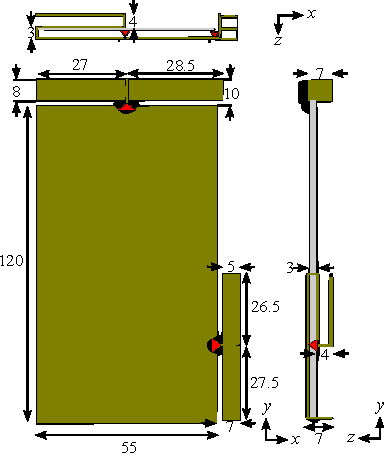
\includegraphics{img/tech_sol/monopole/tech_drawing}
        \caption{Technical drawing.}
        \label{fig:ant1technical}
    \end{subfigure}
    \hfill
    \begin{subfigure}[b]{0.49\linewidth}
        \centering
        \includegraphics{img/tech_sol/schematic_tuning_1}
        \caption{Tuning/matching circuit.}
        \label{fig:ant1schematic}
    \end{subfigure}
    \caption{Technical drawing and tuning circuit for the antenna.  The antennas are built on FR-4 board using \SI{35}{\micro\meter} copper. There is a matching circuit as shown for each of the two feeds.}
    \label{fig:ant2techschem}
\end{figure}

The component values of the matching circuit for both the bottom and side antenna are provided in Table \ref{tab:ant1_matching}.
\begin{table}[]
\centering
\begin{tabular}{|l|l|l|}
\hline
      & $C_1$    & $L_1$    \\ \hline
Ant 1 & 3.017 & 7.996 \\ \hline
Ant 2 & 1.807 & 5.265 \\ \hline
\end{tabular}
\caption{Matching circuit}
\label{tab:ant1_matching}
\end{table}

\begin{figure}[htbp]
    \begin{subfigure}[b]{0.49\linewidth}
        \centering
        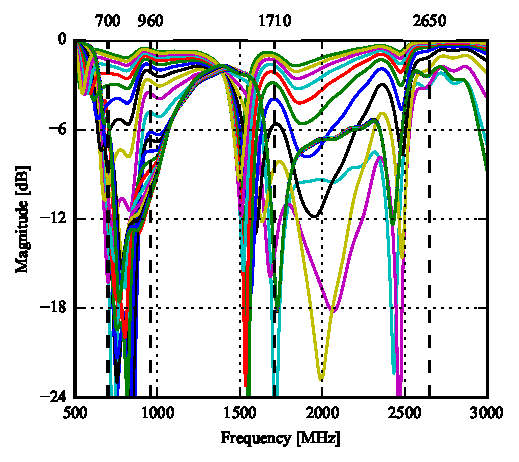
\includegraphics{img/tech_sol/monopole/s11_sweep}
        \caption{S11 plot for the bottom antenna.}
        \label{fig:ant1_s11}
    \end{subfigure}
    \hfill
    \begin{subfigure}[b]{0.49\linewidth}
        \centering
        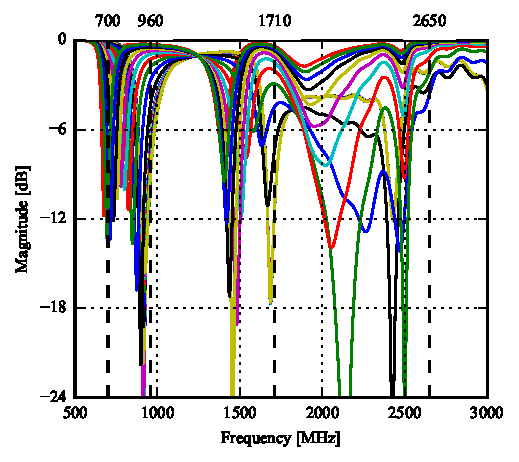
\includegraphics{img/tech_sol/monopole/s22_sweep}
        \caption{S22 plot for the side antenna.}
        \label{fig:ant1_s22}
    \end{subfigure}
    \caption{S11 and S22 results for bottom and side antenna respectively.}
    \label{fig:ant1_sparam}
\end{figure}
The S11 and S22 sweeps \ref{fig:ant1_sparam} shows that both antennas covers the desired bandwidth specified in the requirements \ref{cha:reqspec}. However at approx. \SI{2500}{MHz} both antennas are \SI{-1}{dB} to \SI{-3}{dB} lower than required. The return loss from the bottom antenna \ref{fig:ant1_s11} also have a lower value at approx. \SI{1900}{MHz}. From the requirement specification \ref{cha:reqspec} it is specified that for the low band the minimum channel bandwidth should be \SI{80}{MHz} and for the high band \SI{720}{MHz}. The channel bandwidth for both antennas are shown in Table \ref{tab:asd}     


\begin{figure}[htbp]%{0.49\linewidth}
  \centering
  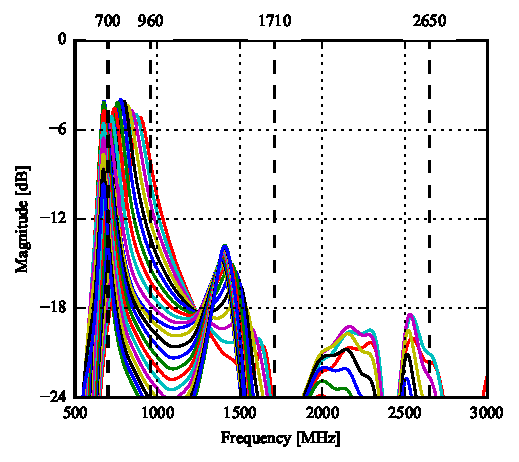
\includegraphics{img/tech_sol/monopole/s21_sweep}
  \caption{S21 plot}
  \label{fig:ant1_s21}
\end{figure}



